\documentclass{article}

\usepackage{graphicx}
\usepackage{tikz}
\usepackage{tikzsymbols}
\usetikzlibrary{calc,patterns,shapes.geometric}
\pagestyle{empty}
\usepackage[margin=0pt]{geometry}
\geometry{papersize={14in,12in}}

\def\centerarc[#1](#2)(#3:#4:#5){\draw[#1] ($(#2)+({#5*cos(#3)},{#5*sin(#3)})$) arc (#3:#4:#5);}

\begin{document}
	\begin{figure}
		\centering
		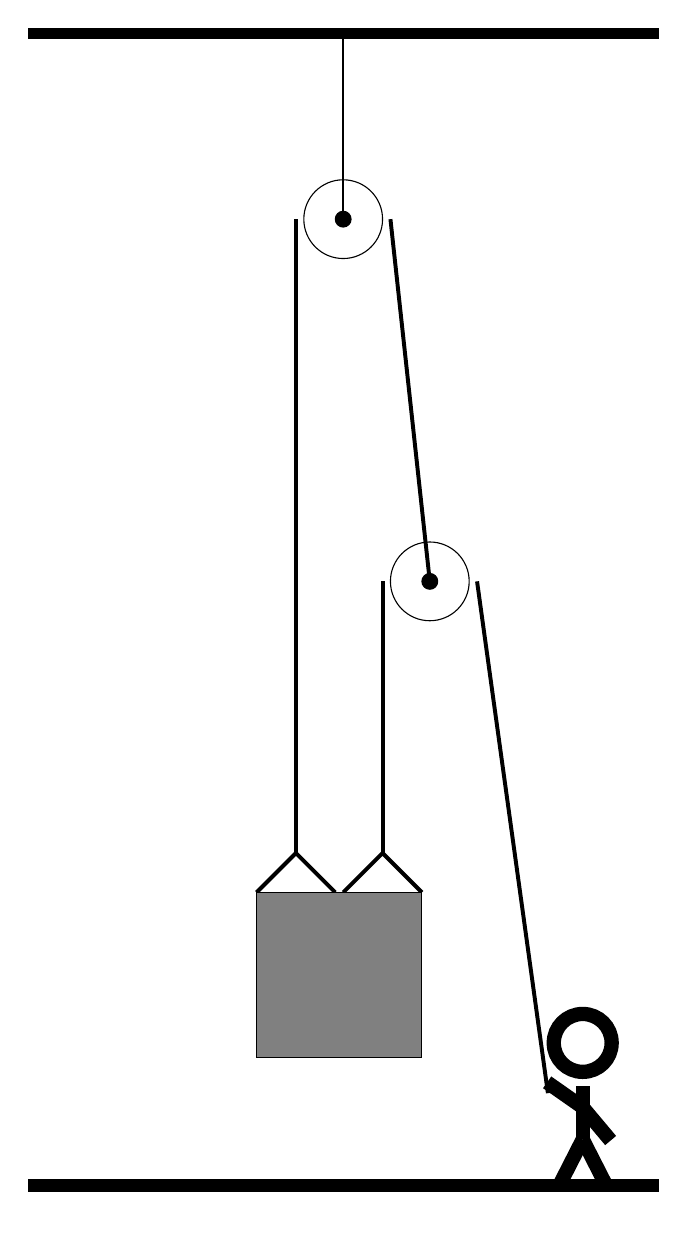
\begin{tikzpicture}
			%%%%% START %%%%%
			\draw[fill=black] (-2, 11.5) rectangle (6, 11.625);
			
			\draw (2, 9.2) circle (0.5);
			\draw[fill=black] (2, 9.2) circle (0.1);
			\draw[thick] (2, 9.2) -- (2, 11.5);
			
			\draw (3.1, 4.6) circle (0.5);
			\draw[fill=black] (3.1, 4.6) circle (0.1);
			
			\draw[line width = 0.5mm]  (0.9, 0.65) -- (1.4, 1.15) -- (1.9, 0.65);
			\draw[line width = 0.5mm]  (2.0, 0.65) -- (2.5, 1.15) -- (3.0, 0.65);
			\draw[fill=black!50] (0.9, 0.65) rectangle (3.0, -1.45);
			
			\draw[line width = 0.5mm] (1.4, 9.2) -- (1.4, 1.15);
			\centerarc[line width = 0.5mm](2, 9.2)(0:180:0.6);
			\draw[line width = 0.5mm] (2.6, 9.2) -- (3.1, 4.6);
			\draw[line width = 0.5mm] (2.5, 4.6) -- (2.5, 1.15);
			\centerarc[line width = 0.5mm](3.1, 4.6)(0:180:0.6);
			\draw[line width = 0.5mm] (3.7, 4.6) -- (4.6, -1.9);
			
			\node at (5, -2) {\Strichmaxerl[10][-35][-50]};
			
			\draw[fill=black] (-2, -3) rectangle (6, -3.15);
			%%%%% END %%%%%
		\end{tikzpicture}
	\end{figure}	
\end{document}